\documentclass{article}

\usepackage{amsmath,amssymb,amsthm}

\usepackage{graphicx}
\graphicspath{ {./img/} }

\usepackage{biblatex}
\addbibresource[
    style=authoryear
]{resources.bib}

\newtheorem{thm}{Theorem}
\newtheorem{def}{Definition}
\newtheorem{lem}{Lemma}
\newtheorem{proof}{Proof}
\newtheorem{rk}{Remark}
\newtheorem*{lemm*}{Lemma}
\newtheorem*{variants}{}
\newtheorem*{var}{}

\renewcommand{\Rn}[1][n]{\mathbb{R}^{#1}}
\newcommand{\Absbars}[1]{\left\lVert#1\right\rVert}
\newcommand{\rmfd}[1]{Riemannian manifold}
\newcommand{\angle}[1]{\langle #1 \rangle}

\title{Ch. 12: The Energy of a Path}
\author{Nicolas Trutmann}
\date{}

\begin{document}
\maketitle


We'll prove what would seem intuitive, namely that geodesics are minima of both length and energy of
a path between 2 points. That is the project we're working towards.

that was kind of the point of geodesics in the first place. They were defined with the intent of
making a 'minimal path' between two points; an analogue of the straight line in $\Rn$.

Let's give a definition:

\begin{def}[Energy of a Path]
Let $\omega : \Rn[] \rightarrow M $ be a path on a \rmfd, with $\omega(a) = p$ and $\omega(b) = q$.
I.e. $\omega \in \Omega_{p,q}(M)$
\[ E_a^b(\omega) = \int_a^b \Absbars{\frac{d\omega}{dt}}^2 dt \]

We leave off the indices for curves parametrized on $[0,1]$, so $E = E_0^1$.
\end{def}

\subsection{the proportional to arclength argument}

a problem with curves is that we could parametrize them arbitrarily badly.

\begin{def}
    \label{def:reparametrization}
    We say a curve $\gamma$ is
\end{def}





\subsection{sleight of hand: calculus of variations}

\newcommand{\OM}{\Omega(M)}
The big cheat of these chapters is that we're able to do calculus on $\OM$.
This is a priori not a manifold, topological space, vector field or group.
It becomes, however, after doing some math to it.

In Milnor's book \cite{milnor}, this problem is explicitly brushed under the table.
Books that treat the matter more thoroughly brush it under the table with a few more words
\cite{salamon}.
Here is a reference that is explicit and thorough: \cite{lee}

Since Milnor hand-waves the problem, so will we. Since we still need intuition for what we're
skipping I provide here two pictures, which we will pretend is how all the curves under scrutiny
look like.

\begin{figure}
    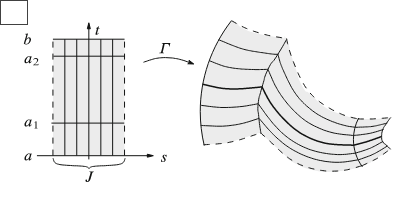
\includegraphics{img/grid.png}
    \caption{grid shape}
    \label{fig:boat1}
\end{figure}
\begin{figure}
    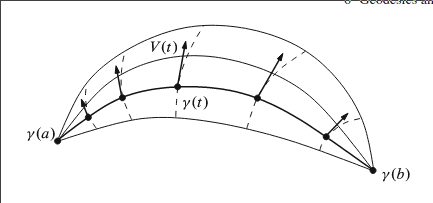
\includegraphics{img/sail.png}
    \caption{variation}
    \label{fig:boat1}
\end{figure}



What we'll need in particular is the vector field along a variation.

Reminder:

\begin{def}
\label{def:vel_of_var}
    The velocity of a variation $\alpha: (-\epsilon, \epsilon) \rightarrow \Omega(M;p,q)$ with
    $\alpha(0) = \omega$ is defined as

    \[ W_t = \frac{d\alpha}{du}(0)_t \]

    It is the vector field along $\omega$ with $W \in T\Omega_{\omega}$.
\end{def}
\subsection{Theorem 12.1}


Recall:
\[
    \begin{align*}
        W_t &= \frac{d\alpha}{du} \quad\text{derivative of the variation} \\
        V_t &= \frac{d\omega}{dt} \quad\text{velocity of $\omega$} \\
        \Delta_tV &= V_{t+} - V_{t-} \quad\text{discontinuity in the velocity vector} \\
        A_t &= \frac{D}{dt} \frac{d\omega}{dt} \quad\text{acceleration of $\omega$} \\
    \end{align*}
\]

$\Delta_tV = 0$ for all but finitely many points.


\begin{thm}[Milnor's 12.1]
    \label{thm:12.1}

    For a one-parameter variation $\alpha$ of $\omega$, we have:

    \[
        \frac{1}{2} \frac{dE(\alpha(u))}{du} =
        \sum_{k} \angle{ W_t, \Delta_tV } \ \ + \ \ \int_0^1 \angle{ W_t, A_t }
    \]

\end{thm}

As a reminder without proof, a lemma from the book.

\begin{lemm*}[Lemma 8.3]
    For a compatible connection (read: Levi-Civita) and any vector fields $V,W$ along a curve
    $\gamma$, we have
    \[
        \frac{d}{dt}\langle V, W \rangle   =
        \langle \frac{DV}{dt}, W \rangle + \langle V, \frac{DW}{dt} \rangle
    \]
\end{lemm*}



\begin{proof}[\ref{thm:12.1}]
    To begin the proof let's talk about the intuition of what we're writing down here.

    What we care about in this equation is not the equation itself, but when it is zero. We are
    searching for extremal points of our variation.

    The first part of the equation tells us what we can expect from "kinks" in our curve. They will
    add to the derivative, which suggests that kink-free or smooth curves are candidates for
    geodesics.

    The second part concerns the acceleration must be orthogonal to $W_t$ to be identically zero.
    The intuitive interpretation is that our curve may not curve.

    Together with the fact that the velocity $V_t$ is constant it follows that the acceleration is
    normal on the tangent space.


    The proof itself follows from a very direct computation.


    Take the left-hand side and insert definitions.

    \[
        \frac{1}{2} \frac{dE(\alpha(u))}{du} =
        \frac{d}{du} \int_0^1 \angle{\frac{\partial \alpha}{\partial t}, \frac{\partial \alpha}{\partial t}} =
        2 \int_0^1 \angle{\frac{D}{du} \frac{\partial \alpha}{\partial t}, \frac{\partial \alpha}{\partial t}}
    \]

    By Lemma 8.5 we can substitute
    $\frac{D}{dt} \frac{\partial \alpha}{\partial u}$ for
    $\frac{D}{du} \frac{\partial \alpha}{\partial t}$ in this last formula.

    Next, we partition $t$ at the discontinuous parts into $0 \lt t_1 \lt \ldots \lt t_k \lt 1$,
    such that $\alpha$ is differentiable on the intervals $[t_i, t_{i+1}]$.

    On these intervals we do "integration by parts" of sorts, by using the identity

    \[
        \frac{d}{du} \angle{\frac{\partial \alpha}{\partial u}, \frac{\partial \alpha}{\partial t}} =
        \angle{\frac{D}{\partial u} \frac{\partial \alpha}{\partial t}, \frac{\partial \alpha}{\partial t}}
        +
        \angle{\frac{\partial \alpha}{\partial t}, \frac{D}{\partial u} \frac{\partial \alpha}{\partial t}}
    \]

    this implies

    \[
        asdf
    \]

\end{proof}



\subsection{Examples and edgecases}


Hyperbolic space

Projective space



\subsection{The Characterization Theorem}

Grabbed this theorem from another book (\cite{salamon} 4.1.4).
We have done about the same work, just in a different order.
It works as a nice summary here.

\begin{thm}[Characterization of Geodesics]
    Let $I = [a, b] \subset \Rn[]$ be a compact interval and let $\gamma : I \rightarrow M$ be a
    smooth curve. Then the following are equivalent.
    \begin{enumerate}
    \item γ is an extremal of the energy functional, i.e. every variation {γs}s∈R
        of γ with fixed endpoints satisfies
        d
        ds
        ∣
        ∣s=0 E(γs) = 0.
    \item γ is parametrized proportional to the arclength, i.e. the veloc-
        ity |  ̇γ(t)| ≡ c ≥ 0 is constant, and either γ is constant, i.e. γ(t) = p = q for
        all t ∈ I, or c > 0 and γ is an extremal of the length functional, i.e.
        every variation {γs}s∈R of γ with fixed endpoints satisfies
        d
        ds
        ∣
        ∣s=0 L(γs) = 0.
    \item The velocity vector of γ is parallel, i.e. ∇  ̇γ(t) = 0 for all t ∈ I.
    \item The acceleration of γ is normal to M , i.e.  ̈γ(t) ⊥ Tγ(t)M for all t ∈ I.
    \end{enumerate}
\end{thm}





\printbibliography

\end{document}
